\section{Optimizations}

Modern SAT solvers use many advanced optimizations and heuristics to improve the solving time.
However these are usually designed for general problem instances.
With additional knowledge about a specific problem we can try to come up with better rules which lead to decrease of solving time.

In this section we will describe several optimizations that we implemented and evaluated.
Some of these involve a simple change in output instance generation, others involve changes to the SAT solvers themselves.

\subsection{Expression encoding}
The automatic and transparent conversion from unmodified source code to SAT instance via operator overloading and boolean circuits may lead to suboptimal encoding of various expressions.
For example, the \emph{choice} round function in \emph{SHA-1}
\[
Ch(x, y, z) = (x \land y) \oplus (\overline{x} \land z)
\]
leads to an encoding with three variables and ten clauses (three clauses for each \emph{and} gate and four for the \emph{xor} gate) if we apply the Tseitin transformation directly.
A better encoding using just six clauses and one variable is shown in \cite{nossum2012sat}.
In fact, it is possible to encode this expression with just four clauses.
%TODO insert the encodings to demonstrate?

%TODO move to section2 (library) after tseitin/boolean?
To solve this issue we provide an expression optimization function in our library.
Any $n$-ary expression can be wrapped using this function to replace the standard Tseitin encoding with a (potentially) smaller one, in terms of number of extra variables and clauses required.

%> posthocTGH(y=raw[raw$rounds>12,]$time, x=raw[raw$rounds>12,]$label, method='games-howell')
%          n means variances
%s3esno  949   7.4        50
%s3esxor 949   8.2        54
%s3nono  949   7.5        45
%s3noxor 949   8.5        49
%
%                   t   df      p
%s3esno:s3esxor  2.56 1892 0.0521
%s3esno:s3nono   0.52 1891 0.9540
%s3esno:s3noxor  3.63 1896 0.0016
%s3esxor:s3nono  2.11 1878 0.1499
%s3esxor:s3noxor 0.98 1891 0.7581
%s3nono:s3noxor  3.21 1892 0.0075

\begin{figure*}
\centering \begin{tabular}{ccrccrr}
\multicolumn{2}{c}{\textbf{Optimizations}} & \multicolumn{1}{c}{\textbf{Time}} & \multicolumn{2}{c}{\textbf{Optimizations}} & \multicolumn{2}{c}{\textbf{Time}} \\
\textbf{$\chi$ step} & \textbf{$\theta$ step} & \multicolumn{1}{c}{\textbf{Mean}} & \textbf{$\chi$ step} & \textbf{$\theta$ step} & \textbf{t} & \textbf{p}\\ \hline
\xmark & \xmark & $7.5$ & \xmark & \cmark & $3.21$ & $<0.01$ \\
& & & \cmark & \xmark & $0.52$ & $0.95$ \\
& & & \cmark & \cmark & $2.11$ & $0.15$ \\ \hline
\xmark & \cmark & $8.5$ & \cmark & \xmark & $3.63$ & $<0.01$ \\
& & & \cmark & \cmark & $0.98$ & $0.75$ \\ \hline
\cmark & \xmark & $7.4$ & \cmark & \cmark & $2.56$ & $0.05$ \\ \hline
\cmark & \cmark & $8.2$ & \\
\end{tabular}
\caption{Pairwise comparison of four \emph{SHA-3-512} optimization combinations using the \emph{Games-Howell} procedure. Only measurements for more than $12$ rounds were used to avoid randomness in timing, for a total of $n=949$ samples per strategy.}
\label{tbl:gh-sha3-opts}
\end{figure*}

To achieve this we first evaluate the expression on all $2^n$ possible inputs to generate a truth table.
This is then processed using an external truth table minimization tool \emph{Espresso}, which generates a list of clauses that can be used to encode this truth table.
%TODO espresso citation
When this expression is used anywhere in the model a node is created in the boolean circuit representation.
It behaves like any other node and can be used in further expressions, however during instance generation the optimized list of clauses is used instead of the na\"{\i}ve Tseitin encoding.

\subsubsection{SHA-1 analysis}
We evaluated the effectiveness of this optimization on preimage attacks on \emph{SHA-1} using the unmodified Tseitin encoding and using the \emph{Espresso} optimizer on both the \emph{choice} and \emph{majority} round functions.
We measured the running time of finding an $8$-bit preimage for $32$-bit input message.
The preimage bits were obtained by hashing random messages to ensure a solution would exist even for instances with reduced number of rounds.
We repeated the experiment multiple times for a total of $5670$ samples for each variant.
 
Figure \ref{fig:opt-sha1-cmp-espresso} shows the mean running times for both instances without optimizations and for ones using \emph{Espresso} minimization.
As we can see the effect of this optimization is quite small and the running times appear to be identical.

%> posthocTGH(y=raw[raw$rounds>20,]$time, x=raw[raw$rounds>20,]$label, method='games-howell')
%          n means variances
%s1espr 4200   2.5       7.4
%s1none 4200   2.6       7.4
%
%                t   df    p
%s1espr:s1none 1.6 8398 0.12

Using the \emph{Games-Howell} post hoc test \cite{games1976pairwise} on instances with more than $20$ rounds (to reduce the effect of randomness when measuring very short time intervals) we do obtain a mean time improvement of $t=1.6$ seconds however at a fairly high significance level of $p=0.12$ which does not give us enough evidence to reject the hypothesis that this optimization leads to no improvement.
%TODO reference G-H

\subsubsection{SHA-3 analysis} 
We performed a similar experiment for the \emph{SHA-3} hash function, finding an $8$-bit preimage on $32$-bit message where the preimage bits again came from randomly generated messages.
We considered two possible optimizations in the round function and tested four variants -- all combinations of turning on or off these two optimizations.
A total of $2000$ samples was collected for each variant.

The first optimization was minimizing the expression $x \oplus (\overline{y} \land z)$ in the $\chi$ step, which is used to fill the $5\times 5$ state matrix $S$ in each round.

The second optimization was in the $\theta$ step, where the $C$ vector is filled using an exclusive or of five different values.
Without optimization this leads to four extra variables and 16 extra clauses.
Using the \emph{Espresso} minimization will lead to 32 clauses but only one extra variable.

Using the \emph{Games-Howell} procedure again we obtain the pairwise comparison shown in figure \ref{tbl:gh-sha3-opts}.

We can see that the \emph{xor} optimization -- which reduces the number of variables but requires twice as many clauses -- in fact leads to higher solving time (mean difference $t=3.21$) at significance level of $p < 0.01$.
Thus the default behavior is more efficient.
On the other hand, from the high p-value of $0.75$ we can't reject the hypothesis that optimizing the $\chi$ step makes no difference at all.

\subsubsection{Discussion}
Even with large number of samples to eliminate the intrinsic randomness in SAT solving times we were unable to reject hypotheses that the tested optimizations do not lead to an improvement.
From this we conclude that they do not provide significant benefits.

While our library provides this optimization feature to users as we saw in our measurements it is not necessary to use it.
Therefore minimal changes to existing, off-the-shelf implementations of hash functions (without the need to identify expressions with non-optimal Tseitin representation) are sufficient to match the hand-optimized instances such as in \cite{nossum2012sat}.

\begin{figure*}	
\centering 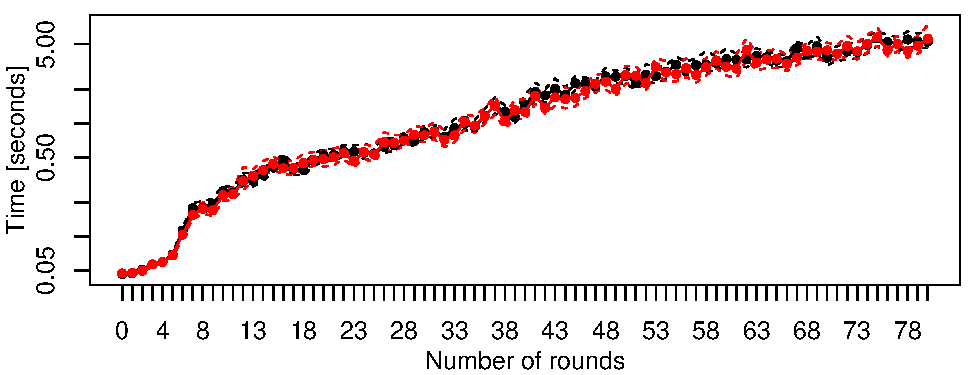
\includegraphics{figures/opt-sha1/sha1-32bit-8bitref-cmp-espresso.pdf}
\caption{Mean running time and 95\% confidence intervals for $8$-bit preimage attack on \emph{SHA-1} without optimizations (black) and using \emph{Espresso} minimization for rounds functions (red).}
\label{fig:opt-sha1-cmp-espresso}
\end{figure*}

\begin{figure*}
\centering 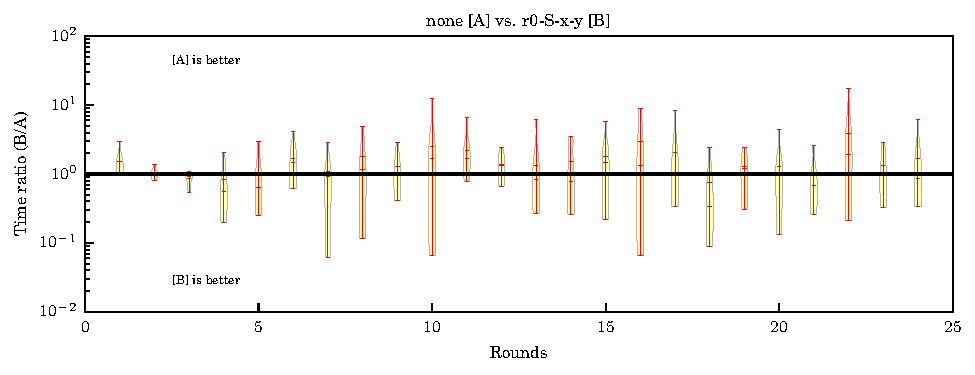
\includegraphics{figures/bo-ex1/ratio-time-none-r0sxy.pdf}
\caption{Violin plot showing the ratios distribution of solving time for the \emph{none} and {r0-S-x-y} strategies.}
\label{fig:bo-ratio-time-none-r0sxy}
\end{figure*}

\begin{figure*}
\centering 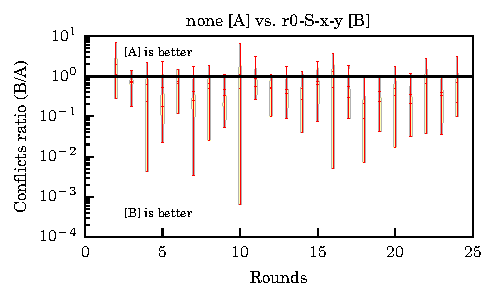
\includegraphics{figures/bo-ex1/ratio-confl-none-r0sxy.pdf}
\caption{Violin plot showing the ratios distribution of number of conflicts for the \emph{none} and {r0-S-x-y} strategies.}
\label{fig:bo-ratio-confl-none-r0sxy}
\end{figure*}

\subsection{Branching order}
\label{sec:branching-order}
%TODO nossum/soos mailing list cite; is it in text?; more references to literature

The most important heuristic in a SAT solver is the decision which unassigned variable to pick next.
A bad order might assign randomly picked values to many variables before some conflict is found and the search tree depth will be quite high.
This in turn leads to an increased solving time.
On the other hand a good heuristic would pick variables in an order that causes many propagations and with an unsatisfiable assignment leads to conflicts quickly.

The branching order is picked by a heuristic in the SAT solver, which does not have additional knowledge about what these variables represent and how they relate to each other.
By extending the input file format and the variable picking algorithm we can provide our own (partial) variable branching order.

\subsubsection{Implementation}
\label{sec:branching-order-impl}
We added a new input line type to the \emph{DIMACS CNF} file format.
A line in the form

\centerline{\texttt{b $v$ 0}}

\noindent means that variable $v$ should be branched on first.
When multiple such lines are provided the order of branching is the same as the order of these lines in the input file.
Using this we can provide a list of any number of variables in the order we want them to be picked for assignment.

We modified the popular \emph{MiniSat} solver \cite{een2005minisat} to be able to parse and store this list.
Then we modified the selection of next branching candidate to first pick all these variables in the specified order.
Once all have been assigned we fall back to the standard branching order algorithm.

We have also added support for this to our modeling library.
Before the boolean circuit is transformed to a set of CNF clauses and written to a file, the user can specify arbitrary branching order using variables defined in the model of the cryptographic primitive.

\subsubsection{SHA-3 analysis}
For \emph{SHA-3-512} we tested various branching orders on $8$-bit reference preimage attack with number of rounds ranging from $0$ to $24$ (full SHA-3).
For every number of rounds 10 different instances were generated and each was solved 10 times, for a total of 100 samples per round per strategy.
We compared the following branching order strategies:

\textbf{\emph{none}}: No branching order was specified. This is the default unmodified \emph{MiniSat} behavior.

\textbf{\emph{r0-S-x-y}}: The $S$ matrix from the first round is branched on first, in column-major order.

\textbf{\emph{r0-S-y-x}}: Same as previous one, but in row-major order.

\textbf{\emph{rlast-S-x-y}} and \textbf{\emph{rlast-S-y-x-}}: Same as previous two, but the $S$ matrix from the last round is used instead.	

The figures \ref{fig:bo-ratio-time-none-r0sxy} and \ref{fig:bo-ratio-confl-none-r0sxy} show \emph{violin plots} of the distribution of ratios of the solving time and the number of conflicts.
Each \emph{violin} also show the mean, median and extreme values.

From these plots we see that while the ratios for the number of conflict are mostly below 1 (meaning that the \emph{r0-S-x-y} strategy leads to fewer conflicts), the time ratios are often higher than 1.

%> posthocTGH(y=confl[confl$rounds>12,]$time, x=confl[confl$rounds>12,]$label, method='games-howell')
%              n means variances
%none        480   731    330234
%r0-S-x-y    480   250     51256
%r0-S-y-x    480   250     51256
%rlast-S-x-y 480   731    330234
%rlast-S-y-x 480   731    330234
%
%                         t  df       p
%none:r0-S-x-y           17 624 1.7e-10
%none:r0-S-y-x           17 624 1.7e-10
%none:rlast-S-x-y         0 958 1.0e+00
%none:rlast-S-y-x         0 958 1.0e+00
%r0-S-x-y:r0-S-y-x        0 958 1.0e+00
%r0-S-x-y:rlast-S-x-y    17 624 1.7e-10
%r0-S-x-y:rlast-S-y-x    17 624 1.7e-10
%r0-S-y-x:rlast-S-x-y    17 624 1.7e-10
%r0-S-y-x:rlast-S-y-x    17 624 1.7e-10
%rlast-S-x-y:rlast-S-y-x  0 958 1.0e+00
%> posthocTGH(y=time[time$rounds>12,]$time, x=time[time$rounds>12,]$label, method='games-howell')
%              n means variances
%none        480   7.8        35
%r0-S-x-y    480   7.5        39
%r0-S-y-x    480   7.5        38
%rlast-S-x-y 480   7.8        36
%rlast-S-y-x 480   7.8        35
%
%                            t  df    p
%none:r0-S-x-y           0.647 956 0.97
%none:r0-S-y-x           0.576 956 0.98
%none:rlast-S-x-y        0.185 958 1.00
%none:rlast-S-y-x        0.032 958 1.00
%r0-S-x-y:r0-S-y-x       0.071 958 1.00
%r0-S-x-y:rlast-S-x-y    0.826 956 0.92
%r0-S-x-y:rlast-S-y-x    0.680 956 0.96
%r0-S-y-x:rlast-S-x-y    0.755 957 0.94
%r0-S-y-x:rlast-S-y-x    0.609 956 0.97
%rlast-S-x-y:rlast-S-y-x 0.153 958 1.00
\begin{figure*}
\centering \begin{tabular}{lrrlrrrr}
\textbf{Strategy} & \textbf{Time} & \textbf{Conflicts} & \textbf{Strategy} & \multicolumn{2}{c}{\textbf{Time}} & \multicolumn{2}{c}{\textbf{Conflicts}} \\
& \multicolumn{2}{c}{\textbf{Mean}} & & \textbf{t} & \textbf{p} & \textbf{t} & \textbf{p} \\ \hline
\emph{none} & $7.8$ & $731$ & \emph{r0-S-x-y} & $0.65$ & $0.97$ & $17$ & $<0.01$ \\
& & & \emph{r0-S-y-x} & $0.58$ & $0.98$ & $17$ & $<0.01$ \\
& & & \emph{rlast-S-x-y} & $0.18$ & $>0.99$ & $958$ & $>0.99$ \\
& & & \emph{rlast-S-y-x} & $0.03$ & $>0.99$ & $958$ & $>0.99$ \\ \hline
\emph{r0-S-x-y} & $7.5$ & $250$ & \emph{r0-S-y-x} & $0.07$ & $>0.99$ & $0$ & $<0.01$ \\	
& & & \emph{rlast-S-x-y} & $0.83$ & $0.92$ & $17$ & $<0.01$ \\
& & & \emph{rlast-S-y-x} & $0.68$ & $0.96$ & $17$ & $<0.01$ \\ \hline
\emph{r0-S-y-x} & $7.5$ & $250$ & \emph{rlast-S-x-y} & $0.76$ & $0.94$ & $17$ & $<0.01$ \\
& & & \emph{rlast-y-x} & $0.60$ & $0.97$ & $17$ & $<0.01$ \\ \hline
\emph{r0-last-x-y} & $7.8$ & $731$ & \emph{rlast-S-y-x} & $0.15$ & $>0.99$ & $0$ & $>0.99$ \\ \hline
\emph{r0-last-y-x} & $7.8$ & $731$ & & & & &  \\
\end{tabular}
\caption{Pairwise comparison of various branching order strategies for \emph{SHA-3-512} using the \emph{Games-Howell} procedure. Only measurements for more than $12$ rounds were used to avoid randomness in timing for a total of $n=480$ samples per strategy.}
\label{tbl:gh-sha3-bos}
\end{figure*}

The \emph{Games-Howell} procedure (figure \ref{tbl:gh-sha3-bos} confirms these findings, with the mean difference for number of conflicts between the \emph{none} and \emph{r0-S-x-y} strategies of $t = 17$ at significance level $p < 0.01$.
However, for the solving time the high p-value does not let us reject the hypothesis that any difference is due to chance.
Note that once again only samples for more than $12$ rounds were included to avoid the strong effect of randomness for instances that solve in very short time.

The \emph{r0-S-y-x} strategy behaves the same as \emph{r0-S-x-y} -- the number of conflicts for every instance is identical and the differences in time are negligible.
On the other hand the strategies starting with the last round's $S$ matrix lead to the same behavior as not providing any branch ordering at all (the \emph{none} strategy).

Similar experiments were performed with the auxiliary vectors and matrices $B, C$ and $D$ with the same results -- enforcing branching order did not lead to better solving times.

\subsubsection{Discussion}

The fact that these branching order do not change the solving time significantly must mean that either their choice does not lead to any forced assignments and conflicts (which is highly unlikely) or that the default \emph{MiniSat} heuristic is also picking them for branching first.
The second case means that this optimization is unnecessary and that the default SAT solver heuristic is sufficient in this case.